\begin{figure*}[!h]
\floatbox[{\capbeside\thisfloatsetup{capbesideposition={right,top},capbesidewidth=8cm}}]{figure}[\FBwidth]
{\caption{Architecture of our best model in relation to BERT. \textbf{Left}: BERT and its span annotation inference process. \textbf{Right}: For our model, BERT embeddings are first transformed through our custom adapter layer. Next, the last two dimensions are flattened. Optionally, a skip connection is added between the sequence outputs of the final BERT layer and this flattened representation. This is present in the best model discovered at 3/10 of an epoch, but was not necessary for the best model discovered at 1 full epoch. This tensor is then projected down to (386, 2) with a densely connected layer, and split on the last axis into two model heads, representing start span position and end span position.}\label{fig:test}}
{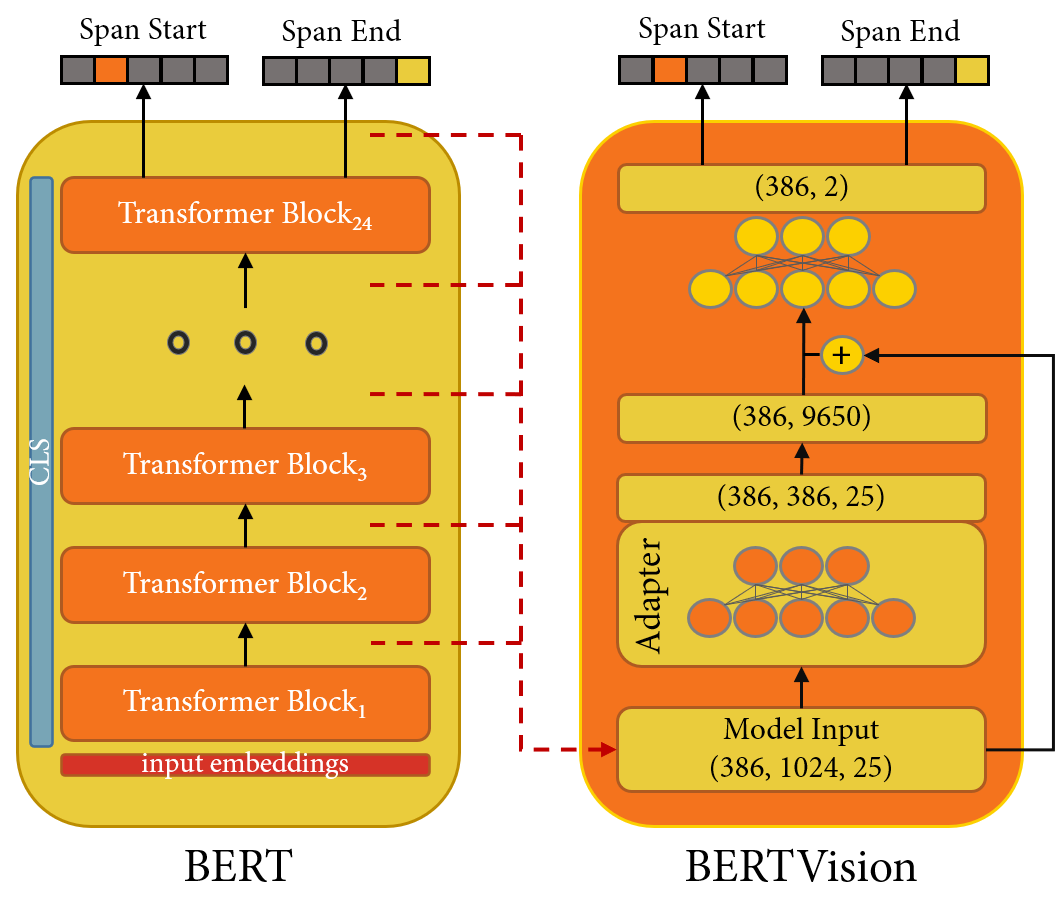
\includegraphics[width=7.5cm]{images/BERTVision_QA_Model.png}}
\end{figure*}